\section{Ceph RADOS Scaling: Initial Results}

RADOS is a reliable distributed object store, the foundational component for
CephFS file system. There are two types of scaling tests we are interested at
the RADOS layer:

\begin{itemize}
  \item scaling on the number of OSD servers
  \item scaling on the number of OSDs per OSD server
\end{itemize}

Our system setup poses some limitations on the scalability tests we wanted to
perform. In particular, we currently had four OSD servers, eight clients, and
eleven OSD servers per client. The scaling tests, therefore, will be within
these constraints.

We used the open-source RADOS Bench tool, developed by Inktank, to perform our
initial performance analysis of the underlying RADOS layer.  RADOS Bench simply
writes out objects to the underlying object storage as fast as possible, and
then later reads those objects in the same order as they were written.

We observed that using two or more client processes and many concurrent
operations are important when performing these tests.  We tested eight client processes 
with 32 concurrent 4 MB objects in flight each. We created a pool for
each RADOS Bench process to ensure that object reads come from independent pools
(RADOS Bench is not smart enough to ensure that objects are not read by multiple
processes and thus possibly cached).  A sync and flush is performed on every
node before every test to ensure no data or metadata is in cache.  All tests
were run with replication set to one.  The backend file systems were XFS,
BTRFS and EXT4 file systems were not tested at this time.


\subsection{Scaling on number of OSDs per server}

In the following test, a single Ceph host drives $n$ OSDs, where $n$ increases
from one to eleven. The result is illustrated in Figure~\ref{fig:osd-scale}.
We ran the test against a single client with four concurrent processes. In this
test case, we observe that the OSD server exhibits near linear scalability up to
nine OSDs, and is still trending upwards at eleven OSDs. This suggests that we
have not reached the saturation point yet. Additional testing would require
provisioning more OSDs on the SFA10K backend.


\begin{figure}[!t]
\centering
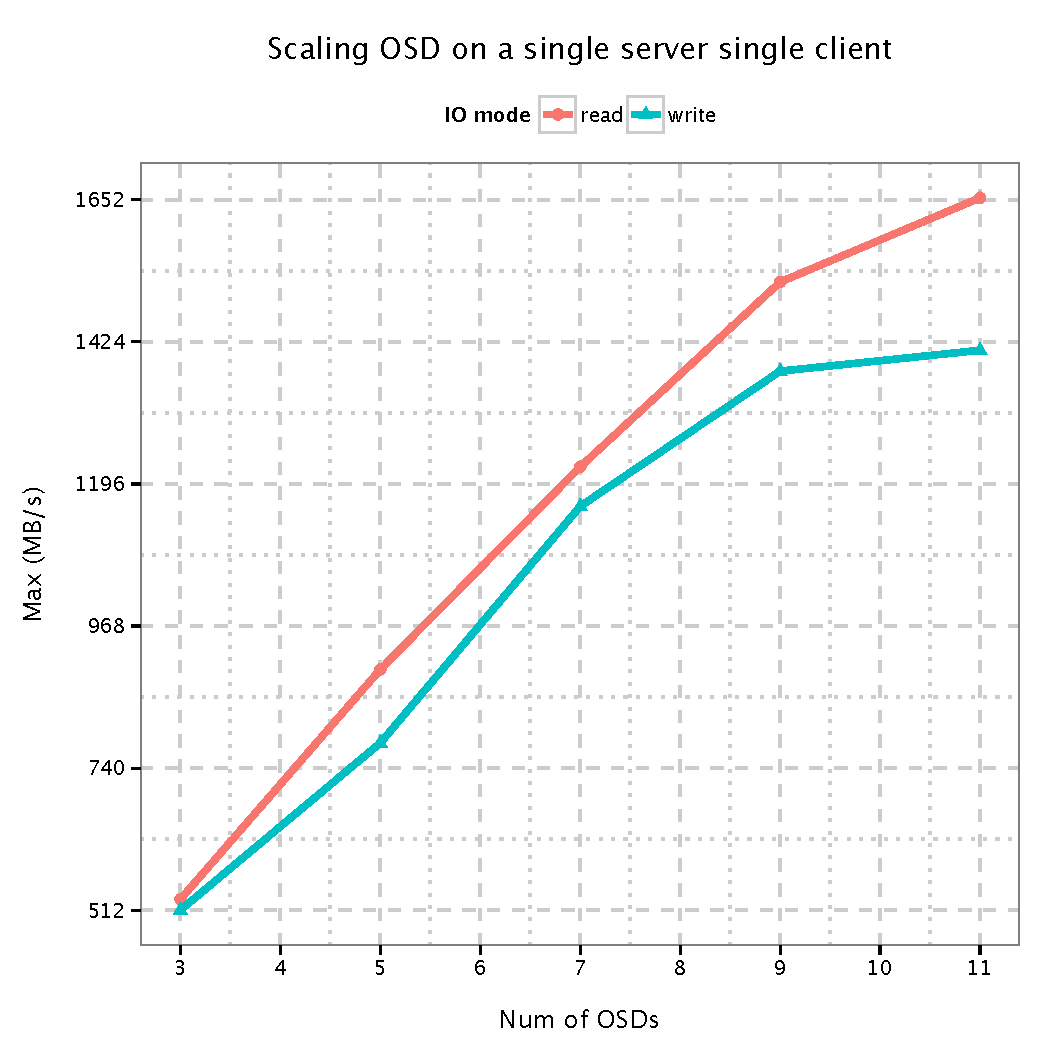
\includegraphics[width=3in]{data/rados_osd}
\caption{RADOS scaling on number of OSDs}
\label{fig:osd-scale}
\end{figure}

\begin{figure}[!t]
\centering
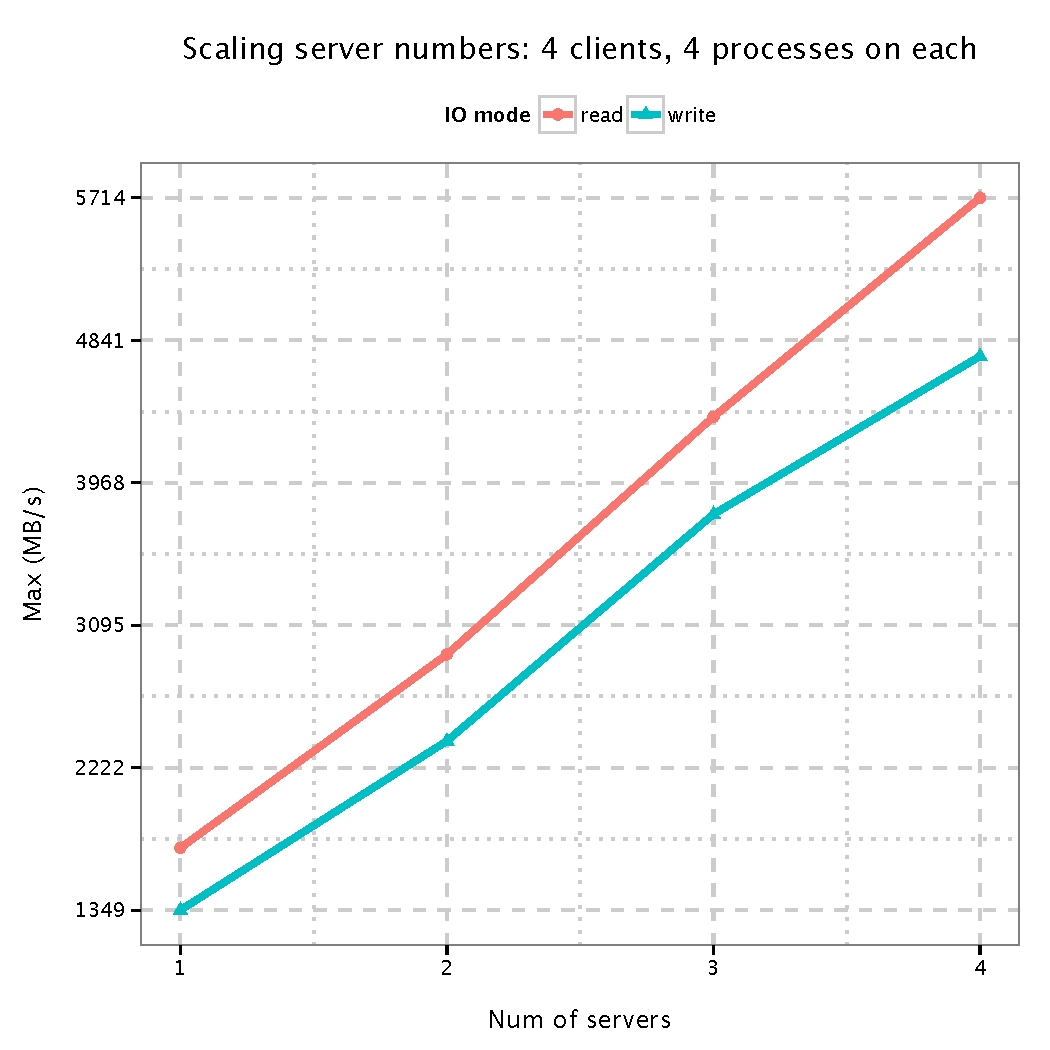
\includegraphics[width=3in]{data/rados_server}
\caption{RADOS scaling on number of servers}
\label{fig:oss-scale}
\end{figure}

\subsection{Scaling on number of OSD servers}

In this test, we exercise OSD servers from one to four, driven by four hosts
each with four RADOS Bench process. Each additional OSD server
adds eleven more OSDs into play. We observe that Ceph exhibits linear scaling with
regard to number of servers as well, at least in the given set of servers.
However, the peak performance we are seeing is about the half of what are
expecting from the SFA10K (compare to the baseline block I/O perforamnce number
presented in Section~\ref{sec:block-io}).

For writes, the lost performance is attributed to the way Ceph performs
journaling:
Ceph does not support meta-data only journaling, therefore every write is the
equivalent of a double-write: once to the data device, once to the journaling
device. This effectively cuts the observed system bandwidth in half. That said,
it does not explain the read performance -- it is a little better than write,
but still far from the theoretical maximum.

\section{Ceph File System Performance: Initial Test}
\label{sec:ior-initial}
We used the synthetic IOR benchmark suite for file system level performance and
scalability test.
The particular parameter setup is show in Table \ref{tbl:ior}. Each client node
has 6 GB of physical memory, the block size is set so as to mitigate cache
effects. In addition, the test harness program issues the following commands
at the beginning of each test:




\begin{table}[tb]
\caption{IOR parameter setup}
\label{tbl:ior}
\centering
\begin{tabular}{p{0.8in} | p{2in}}
    \hline
    IOR parameter & Note \\ \hline
    \verb!-F! & file per process \\ \hline
    \verb!-a POSIX! & use POSIX API \\ \hline
    \verb!-w -r -C! & do both write and read test, \verb!-C! is to change task
        ordering for read back so it will not read from the write cache. \\
        \hline
    \verb!-i 3 -d 5! & 3 iterations and delay 5 seconds betewen iterations \\ \hline  
    \verb!-e! & perform \verb!fsync()! upon POSIX write close \\ \hline
    \verb!-b 8g or 16g! & the block size \\ \hline
    \verb!-t 4k to 4m! & the transfer size \\ \hline
    \verb!-o file! & mandatory test file  \\    
    \hline
\end{tabular}
\end{table}


\begin{Verbatim}[fontsize=\small]
# sync
# echo 3 | tee /proc/sys/vm/drop_caches
\end{Verbatim}


Here, 0 is the default value of \verb!drop_caches!; 1 is to free pagecaches, 2
is to free dentries and inodes, 3 is to free pagecache, dentries, and inodes.


Our first round of tests was less than ideal as we encountered various issues. For
the sake of completeness, we first summarize the results, then discuss
further tuning efforts and improvements.

The full permutation of IOR parameters were not explored due to I/O errors we encountered.
We were, however, able to record results in two extreme cases as far as
transfer size is concerned: 4 KB and 4 MB, using a fixed number of OSD servers
(4) and fixed block size (8 GB), the results are illustrated in Figure
\ref{fig:ior4k} and \ref{fig:ior4m}, we make the following observations:


\begin{figure*}[!t]

\centerline{\subfloat[4 KB transfer size]
{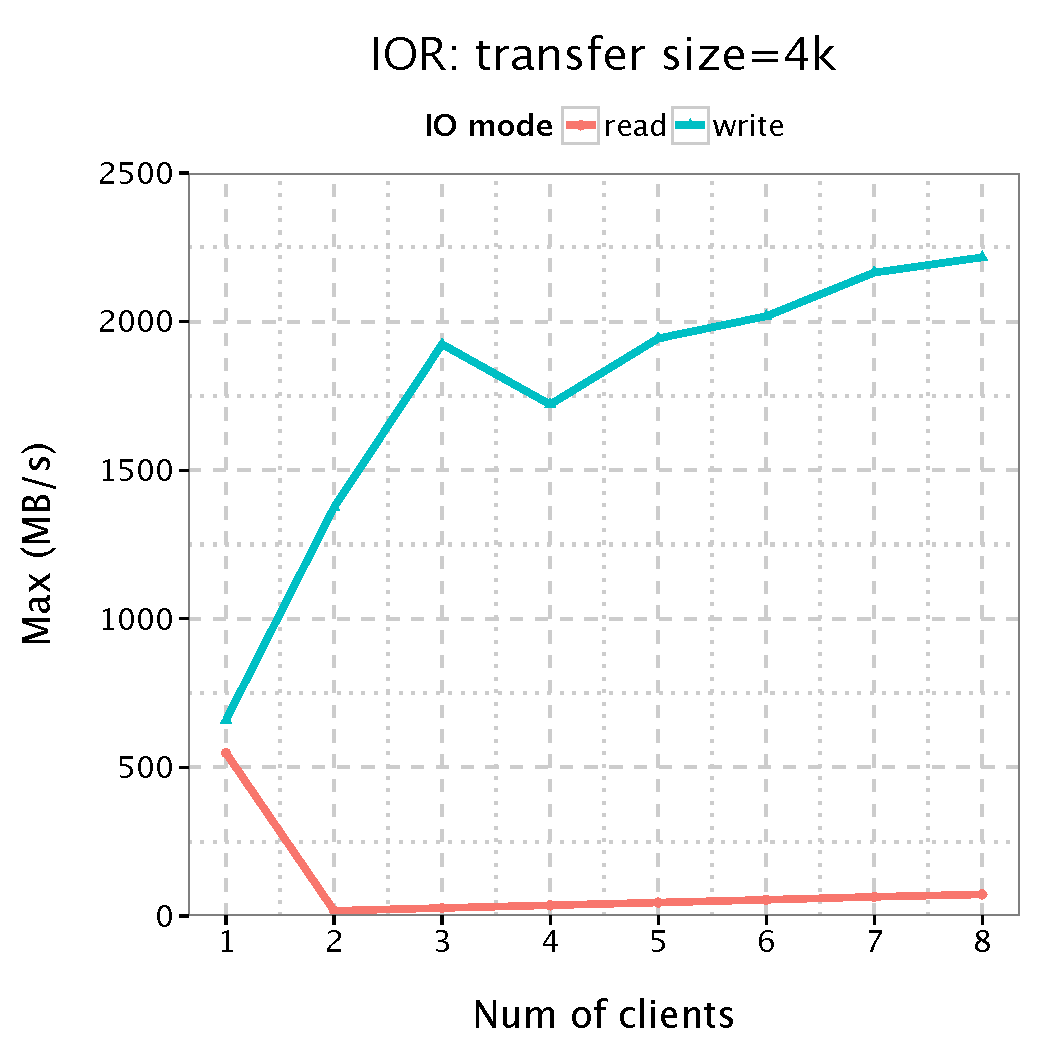
\includegraphics[width=3in]{data/ior_4k}
\label{fig:ior4k}}
\hfil
\subfloat[4 MB transfer size]
{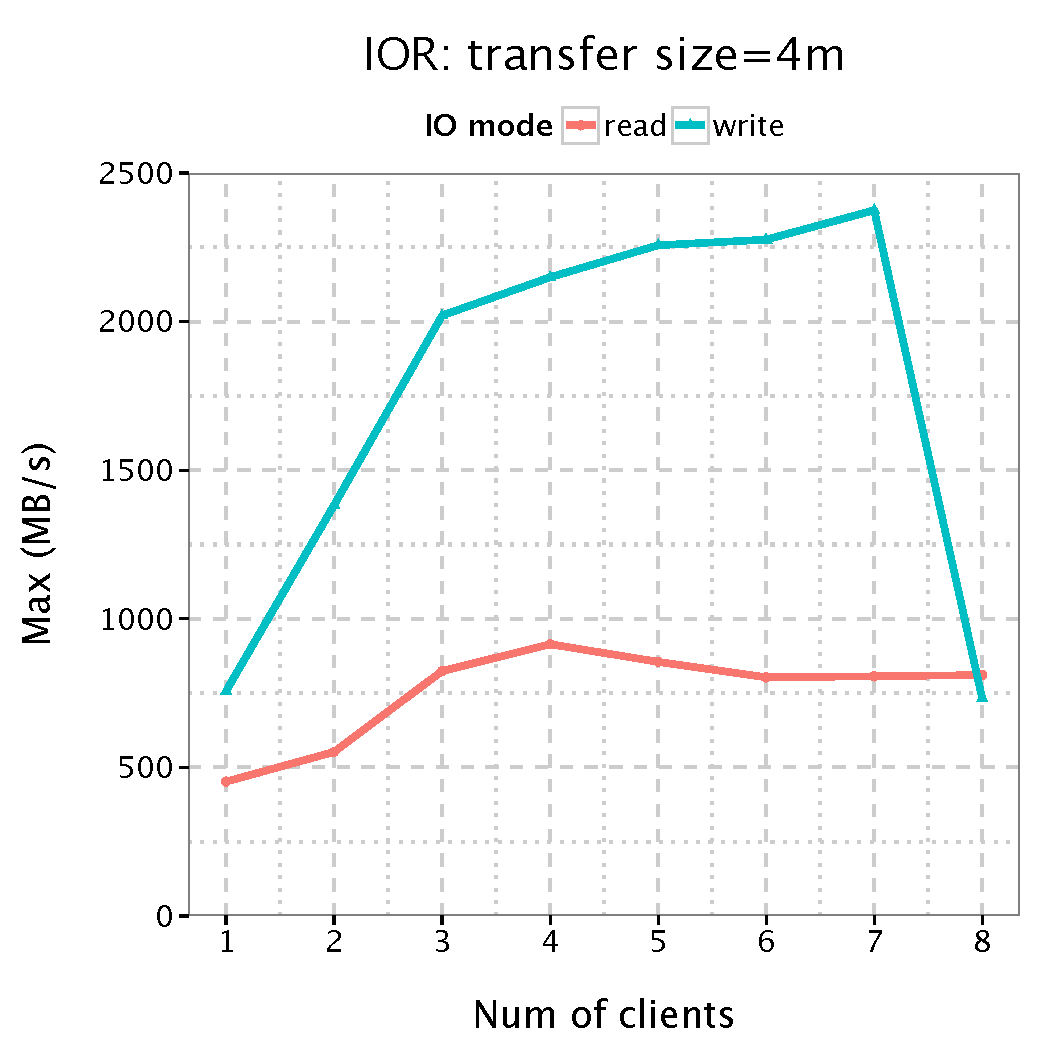
\includegraphics[width=3in]{data/ior_4m}
\label{fig:ior4m}}
}% end of centerline
\caption{CephFS scalability test with IOR}

\end{figure*}


\begin{itemize}

  \item The small read (4 KB transfer size) performance is almost an anomaly
  -- we will investigate why it is so low compare to write performance and
  present improved results in Section~\ref{sec:improve-ior}.

  \item The large read (4 MB transfer size) performance is almost half of the
  RADOS read performance.
   
  \item The write performance is also about half of what we can obtain from
  RADOS Bench. When number of clients reaches 8, there is a significant
  performance drop as well. 

\end{itemize}


We will describe the efforts and results on performance improvement in the
following sections.

